\begin{pastexam}[label={px:ccu-115-swa-13}]{中正資工所甲組 115 學年度 第 23 題}
（複選；全對才給分）

(3\%) (\qquad) Given the following in-order and post-order traversals of a binary tree, reconstruct
the binary tree uniquely determined by these traversals, and then delete node $D$ from the tree.
What is the level-order traversal of the resulting tree after the deletion?

In-order：A, B, G, E, D, I, J, F, H, C\\
Post-order：G, E, J, I, H, F, D, C, B, A\\
(a)~A, B, C, E, F, G, I, H, J \qquad (b)~A, B, G, E, C, I, J, F, H \qquad
(c)~A, B, C, E, G, F, I, J, H\\
(d)~A, B, C, J, E, F, G, I, H \qquad (e)~none of the above
\end{pastexam}

\begin{pastsoln}
答案：(d)（採用的刪除方法見下）。

先說原題的問題：這不是二元搜尋樹（中序不是依字母排好的），「從一般二元樹刪掉一個有兩個子節點
的節點」沒有唯一的標準做法，題目也沒有指定。 選項 (d) 恰好是常見的一種做法的結果：\textbf{拿
最深、最右邊的節點（層序走訪的最後一個）來取代被刪的節點}，再把那個最深的節點拿掉。 這個做法
不改變其他節點的上下關係，樹仍然盡量「滿」，是一般二元樹刪除最常見的寫法。 下面照它作答。

\textbf{重建}（資結書第~7.4~節）：後序的最後一個是根，在中序裡找到根，切成左右子樹，照個數切開
後序，兩邊遞迴。
\begin{enumerate}
\item 全部：後序最後是 A，中序裡 A 在最前面，左子樹空，右子樹是 B G E D I J F H C。
\item 根 B（右子樹後序 G E J I H F D C B 的最後一個），左子樹空，右子樹 G E D I J F H C。
\item 根 C，C 在中序最後，右子樹空，左子樹 G E D I J F H。
\item 根 D，左子樹 G E（後序 G E），右子樹 I J F H（後序 J I H F）。
\item G E｜G E：根 E，G 是左子節點。 I J F H｜J I H F：根 F，左子樹 I J、右子節點 H；
I J｜J I：根 I，J 是 I 的右子節點。
\end{enumerate}
\begin{center}
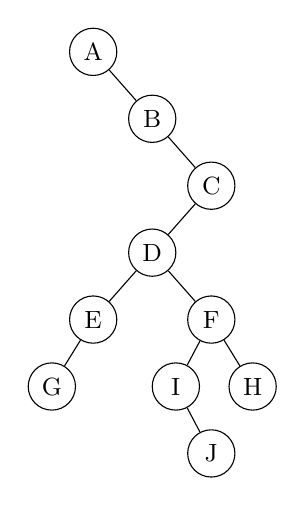
\begin{tikzpicture}[x=0.75cm,y=0.85cm,v/.style={circle,draw,minimum size=6mm,inner sep=0pt,font=\small}]
\node[v] (A) at (0,0) {A};
\node[v] (B) at (1,-1) {B};
\node[v] (C) at (2,-2) {C};
\node[v] (D) at (1,-3) {D};
\node[v] (E) at (0,-4) {E};
\node[v] (F) at (2,-4) {F};
\node[v] (G) at (-0.7,-5) {G};
\node[v] (I) at (1.4,-5) {I};
\node[v] (H) at (2.7,-5) {H};
\node[v] (J) at (2,-6) {J};
\draw (A)--(B) (B)--(C) (C)--(D) (D)--(E) (D)--(F) (E)--(G) (F)--(I) (F)--(H) (I)--(J);
\end{tikzpicture}
\qquad\qquad
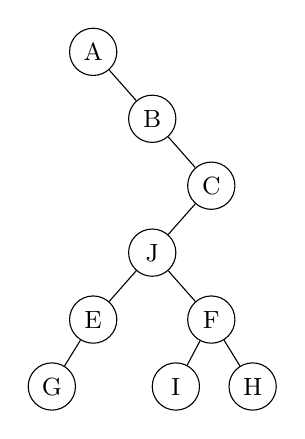
\begin{tikzpicture}[x=0.75cm,y=0.85cm,v/.style={circle,draw,minimum size=6mm,inner sep=0pt,font=\small}]
\node[v] (A) at (0,0) {A};
\node[v] (B) at (1,-1) {B};
\node[v] (C) at (2,-2) {C};
\node[v] (D) at (1,-3) {J};
\node[v] (E) at (0,-4) {E};
\node[v] (F) at (2,-4) {F};
\node[v] (G) at (-0.7,-5) {G};
\node[v] (I) at (1.4,-5) {I};
\node[v] (H) at (2.7,-5) {H};

\draw (A)--(B) (B)--(C) (C)--(D) (D)--(E) (D)--(F) (E)--(G) (F)--(I) (F)--(H);
\end{tikzpicture}
\end{center}
左圖是重建的樹。 檢查：它的中序 A B G E D I J F H C、後序 G E J I H F D C B A 都和題目相同。
原樹的層序是 A, B, C, D, E, F, G, I, H, J，最後一個（最深、最右）是 J。

\textbf{刪除 D}：用 J 取代 D 的位置，再把原來 I 底下的 J 拿掉，得到右圖。 層序走訪（資結書
第~7.3.2~節）一層一層由左到右：A；B；C；J；E, F；G, I, H，也就是
\[
\mathrm{A, B, C, J, E, F, G, I, H},
\]
就是 (d)。

\begin{itemize}
\item (a) 錯：這是原樹的層序直接劃掉 D，不是任何一棵樹的層序：拿掉 D 後 E、F 要有新的父節點，
樹的形狀會變。
\item (b) 錯：中序劃掉 D 再把 C 往前搬，不是層序。
\item (c) 錯：這看起來像是用左子樹裡最右的節點 E（中序前驅）取代 D，但那棵樹的層序是
A, B, C, E, G, F, I, H, J（H 和 I 同一層、J 在下一層），(c) 把 J 排在 H 前面，也不對。 用中序後繼 I
取代 D 則得到 A, B, C, I, E, F, G, J, H，也不在選項裡。
\item (e) 錯，照上面的做法 (d) 對。
\end{itemize}
若閱卷者採用中序前驅或後繼取代，四個選項都不對，答案會變成 (e)；作答時最好把採用的刪除方法
寫出來。
\end{pastsoln}
